\section{Anwendungsbereiche}
In diesem Abschnitte werden einige der aktuellen Anwendungsbereiche von WebGL vorgestellt.
\subsection{Google Maps}
Eine der wohl bekanntesten Beispiele wo WebGL angewendet wird ist Google Maps.
Hierbei profitiert die in Abbildung~\ref{fig:GoogleMaps} gezeigte Satellitenansicht von der dritten Dimension.
Gebäude können dadurch deutlich realitätsnaher dargestellt werden als auf einer einfachen Karte auf der man nur die Umrisse sieht.
\begin{figure}
    \centering
    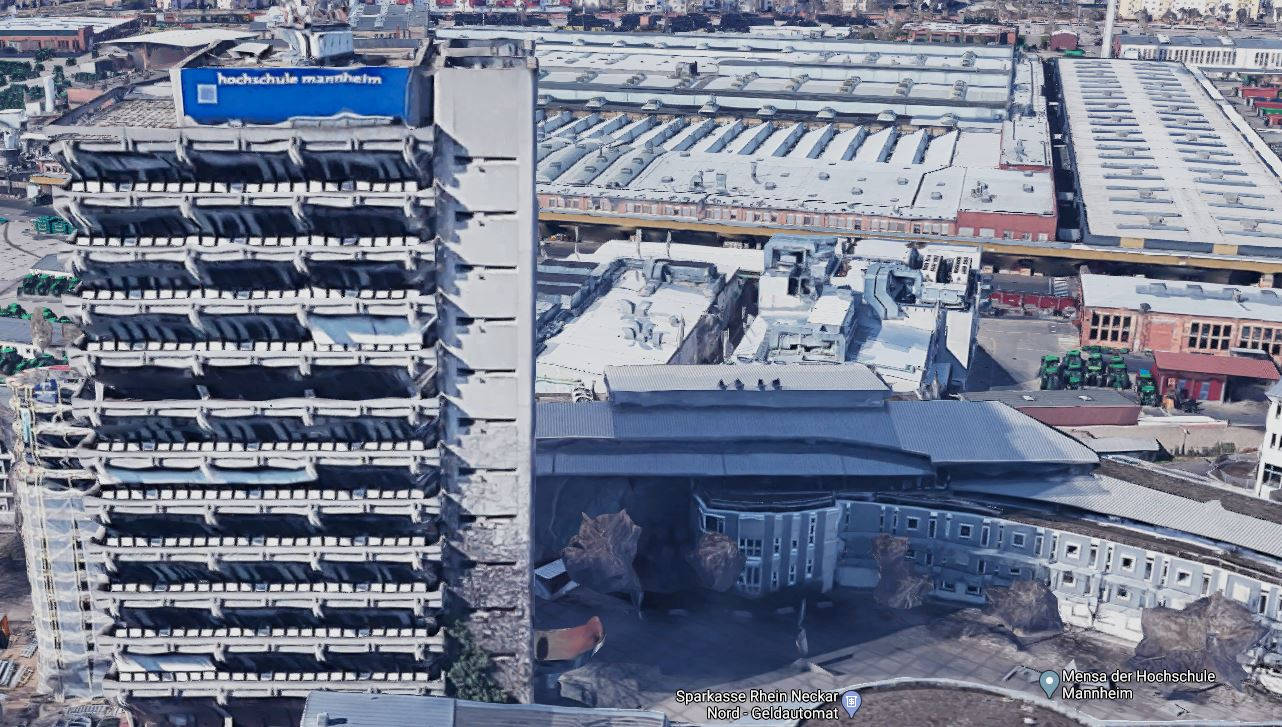
\includegraphics[width=6cm]{GoogleMapsExample.jpg}
    \caption{Google Maps Satellitenansicht\cite{GoogleMaps}} \label{fig:GoogleMaps}
    \end{figure}

\subsection{Online Shopping?~\cite{WebGLExamples2}}
\subsection{3D Entwicklung/ 3D Druck}
\subsection{Videobearbeitung}
\subsection{3D Simulationen~\cite{BioDigital}/Medizin}